\section{Design Phase} \label{designPhase}

\subsection{Third Party Libraries}

\paragraph{Cinder \cite{developers_davis}} \textit{Cinder} is a free, open-source graphics engine for \CPP. It provides a simple way to access OpenGL, ImGui and other tools, such as image loading and saving, optimised rendering in 2D and 3D, and more. I am using \textit{Cinder} for this project instead of doing all the graphics processing with raw OpenGL because it dramatically simplifies the code and reduces the scope for hard-to-fix bugs.

This project uses a modified version of \textit{Cinder} with updated libraries and a few extra features. Most significantly, this modified version includes a much newer version of ImGui and an altered build configuration to fix common compile errors on some platforms.

\paragraph{LibRapid \cite{Davis_LibRapid_Optimised_Mathematics_2023}} \textit{LibRapid} is a high-performance library for mathematical applications, including optimised vector classes, complex number types and general mathematical functions. However, this library's most helpful feature is its support for MPIR and MPFR, which are highly-optimised multi-precision implementations. This will allow floating point calculations with more than 64 bits.

Incorporating an efficient multi-precision implementation into the project could allow for ``infinite'' fractal zooms since traditional floating-point limitations would no longer constrain the software.

Another feature of \textit{LibRapid} used heavily in this project is the compiler- and system-agnostic macro definitions. Useful features like inlining of functions, no-discard specifiers and more are not implemented by all compilers and sometimes work differently on different operating systems. LibRapid implements macros which automatically detect the relevant information and define the most suitable replacement. This isn't strictly required for the project, but it might result in a slight performance improvement and can help reduce bugs.

\paragraph{Cinderbox} Both of the afore mentioned libraries are packaged with \textit{Cinderbox} for simple integration into \textit{CMake} projects.

\paragraph{JSON for Modern \CPP \cite{Lohmann_JSON_for_Modern_2022}} \textit{JSON for Modern \CPP} is a highly intuitive JSON parser for the latest versions of the language. It supports parsing files, saving to files and representing a usable JSON object at runtime, which is necessary for storing the loaded settings.

\paragraph{Thread-Pool \cite{Shoshany_A_C_17_Thread_2021}} The \textit{thread-pool} library implements a multi-threaded queue implementation, where items are dequeued in parallel and executed. This will be used to simplify the rendering process, as well as accelerate it.

\subsection{Library Heirarchy}

\FloatBarrier
\begin{figure*}[htp]
	\centering
	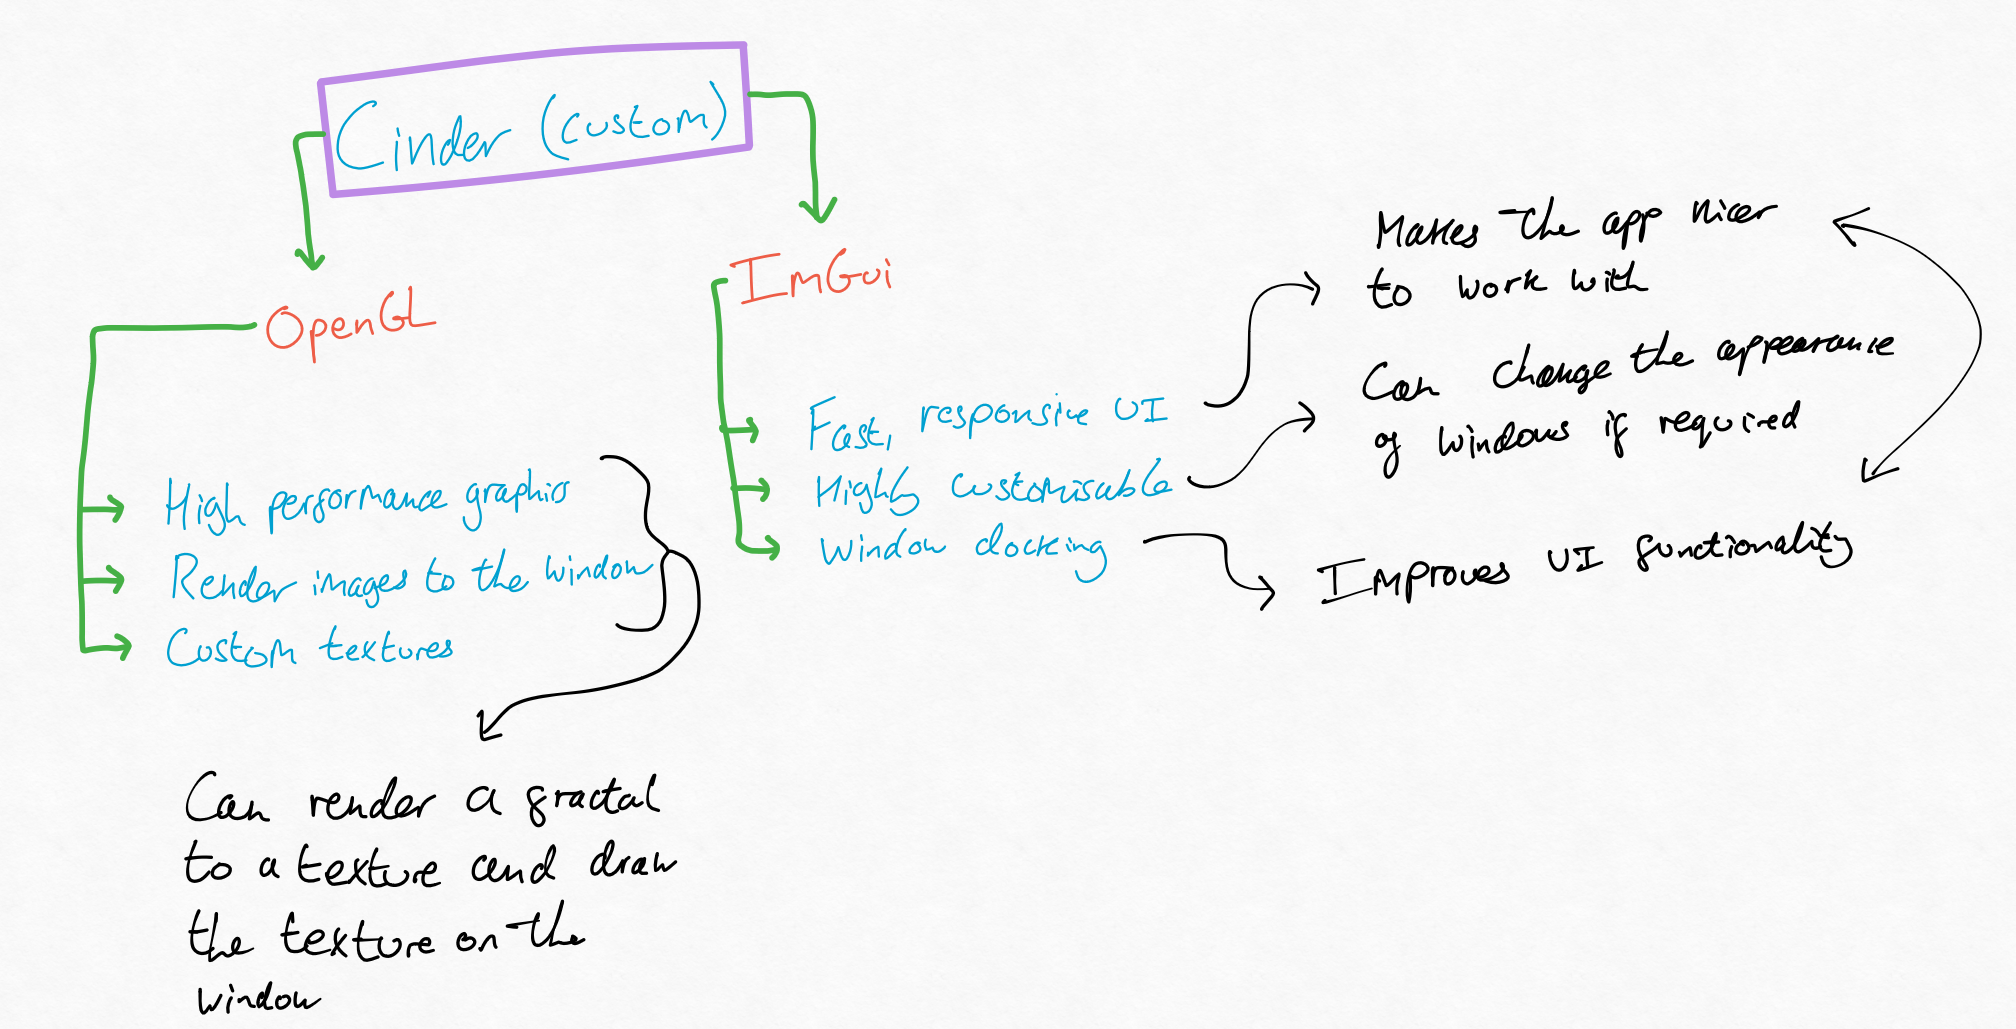
\includegraphics[width=\textwidth]{CinderLibraries.png}
\end{figure*}
\FloatBarrier

\FloatBarrier
\begin{figure*}[htp]
	\centering
	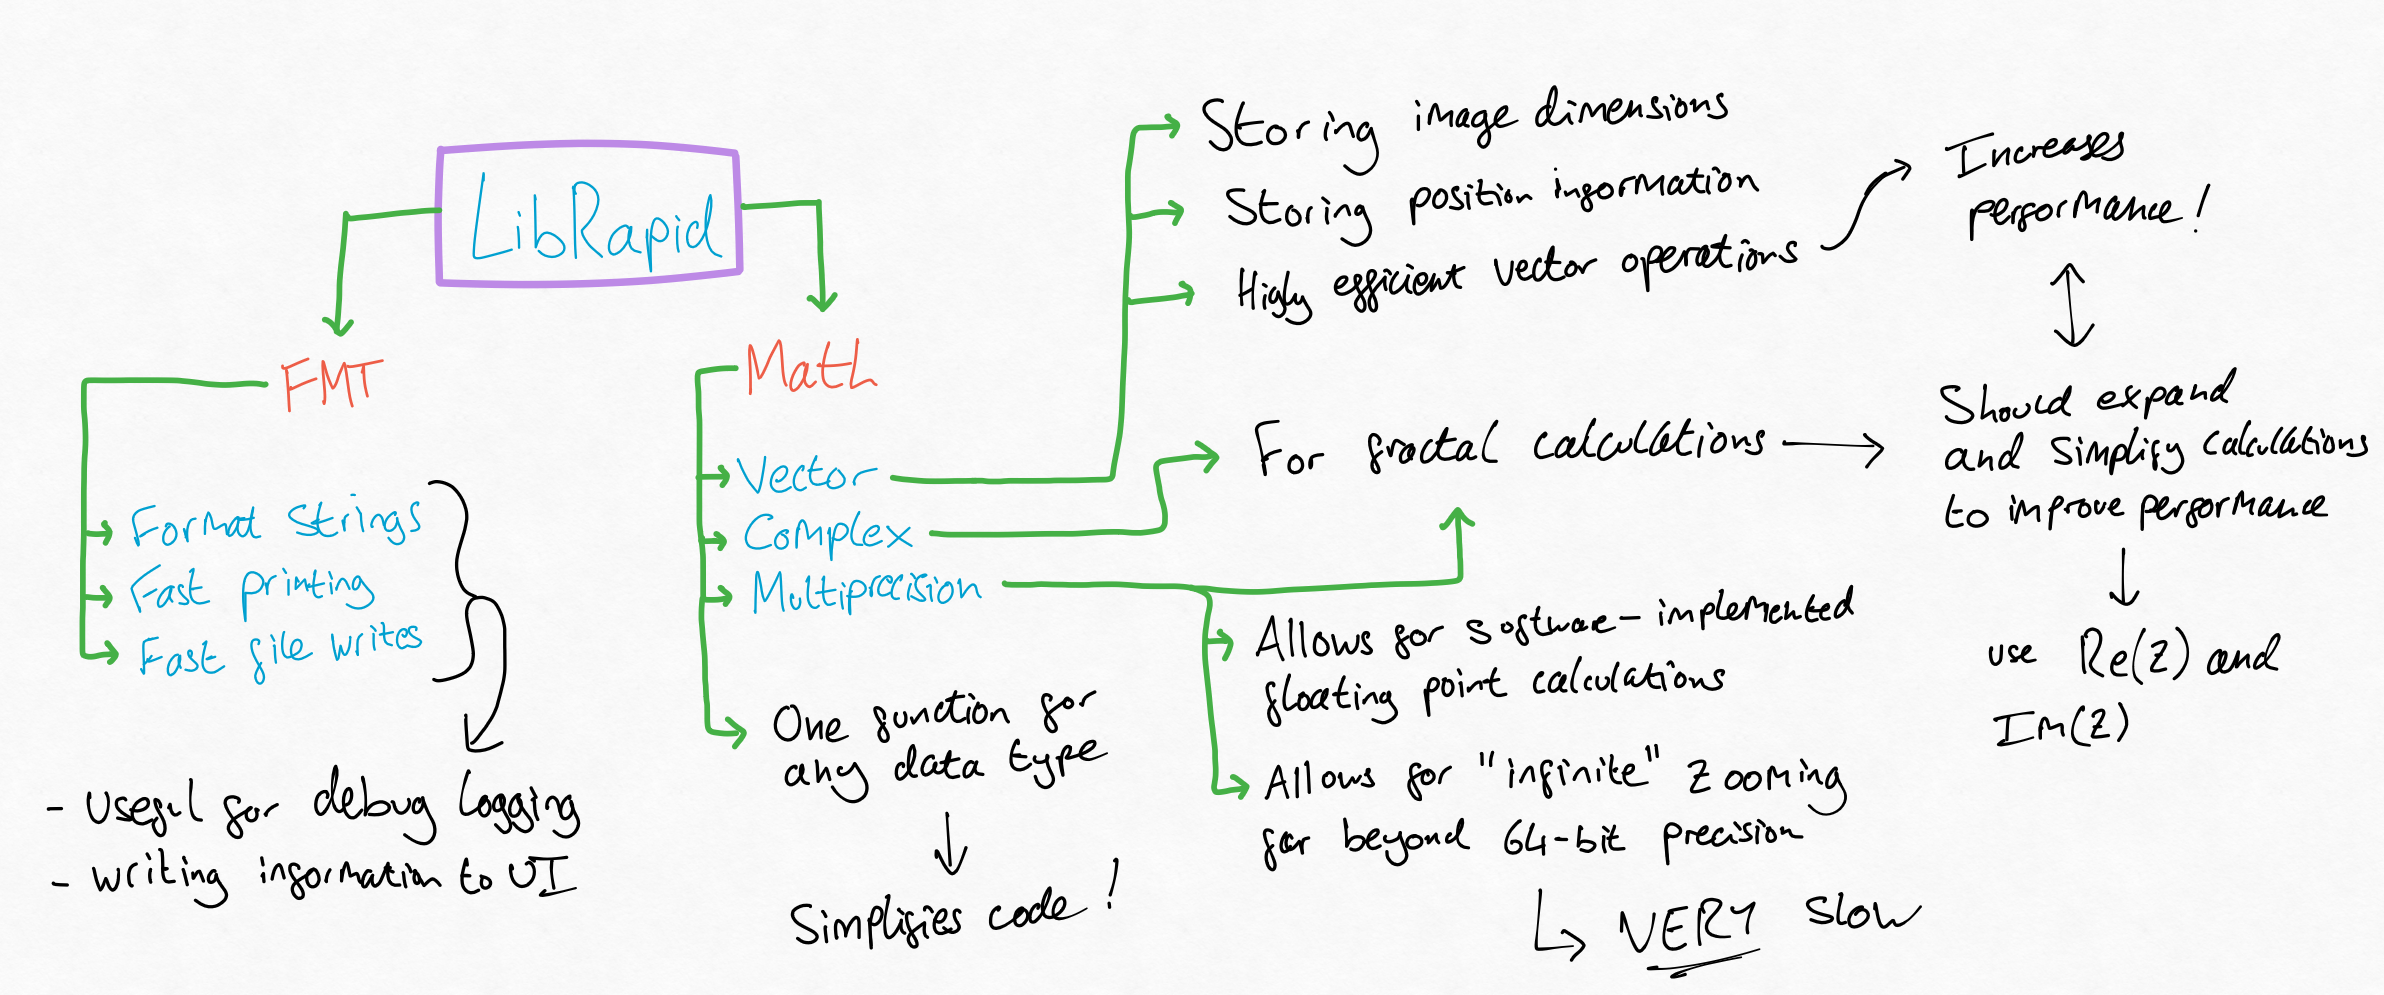
\includegraphics[width=\textwidth]{LibRapidLibraries.png}
\end{figure*}
\FloatBarrier

\subsection{The Debug Logger}

Since the program is written in \CPP and is a GUI application instead of a console application, there will not be a usable standard output to which debug information can be printed. To circumvent this issue, I will use a debug logger instance to write information to a file.

\FloatBarrier
\begin{figure*}[htp]
	\centering
	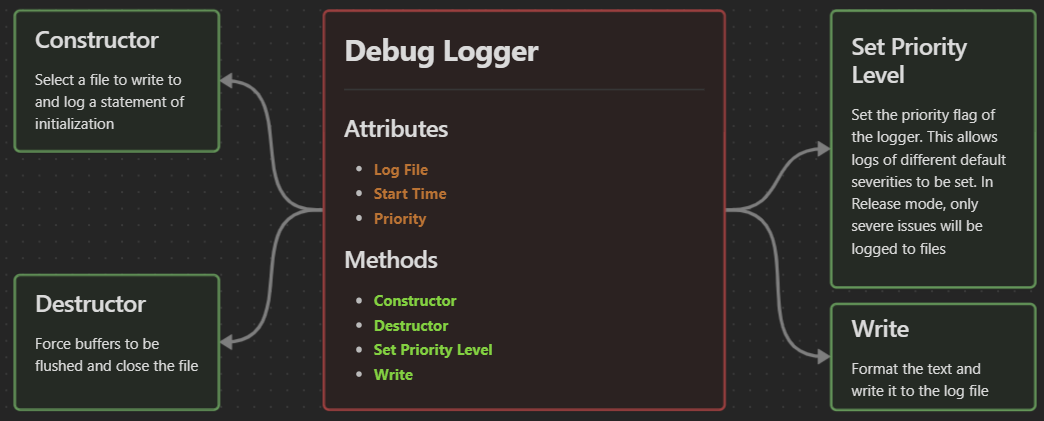
\includegraphics[width=\textwidth]{ClassDebugLogger.png}
\end{figure*}
\FloatBarrier

The logger's constructor will take a file path relative to the executable and attempt to open the specified file. If the document does not exist, it will be created for the user. The destructor will ensure that all buffers are flushed and the file is closed. Without these checks, the program may terminate without saving the changes to be written to the file, and the debug log might be incomplete or corrupt. The logger will also have a priority level, optimising logging in release builds, as the user does not need all the information. For example, the logger could be configured to write only errors to the file in release mode. Finally, the logger has a function which enables the user to send data to be written to the file. New lines should be formatted appropriately, and logs should be timestamped. In addition to these functions, I will create a macro that captures the log statement's line number and filename, making tracebacks easier and faster during development.

\begin{center}
	\begin{tikzpicture}[
		block/.style={rectangle split, rectangle split parts=2, draw, text width=5cm, align=left},
		% arrow/.style={-Stealth, thick}
		]
		
		\node[block] (write) {
			\textbf{write()}
			\nodepart{two}
			$
			\begin{aligned}
				&\text{message} \\
				&\text{priority} \\
				&\text{filename} \\
				&\text{line number}
			\end{aligned}
			$
		};
		
		\node[block, right=1.5cm of write] (filter) {
			\textbf{Priority Filter}
			\nodepart{two}
			Check if message priority is below the set threshold
		};
		
		\node[block, below=1.5cm of write] (format) {
			\textbf{Format Message}
			\nodepart{two}
			Truncate filename \newline
			Get priority string \newline
			Clean and pad message
		};
		
		\node[block, right=1.5cm of format] (log) {
			\textbf{Write to Log}
			\nodepart{two}
			Write formatted message to log file with timestamp and line number
		};
		
		\draw[arrow] (write.east) -- (filter.west);
		\draw[arrow] (filter.south) -- ++(0, -1.25cm) -| (format.north);
		\draw[arrow] (format.east) -- (log.west);
		
	\end{tikzpicture}
\end{center}

\subsection{Colour Palettes}

A simple class containing a list of colours and a few helper methods helps store the colours and gradients used by the fractal rendering process. This class simplifies the act of colour palette generation and usage throughout the software, reducing bugs and improving the rate of development.

\FloatBarrier
\begin{figure*}[htp]
	\centering
	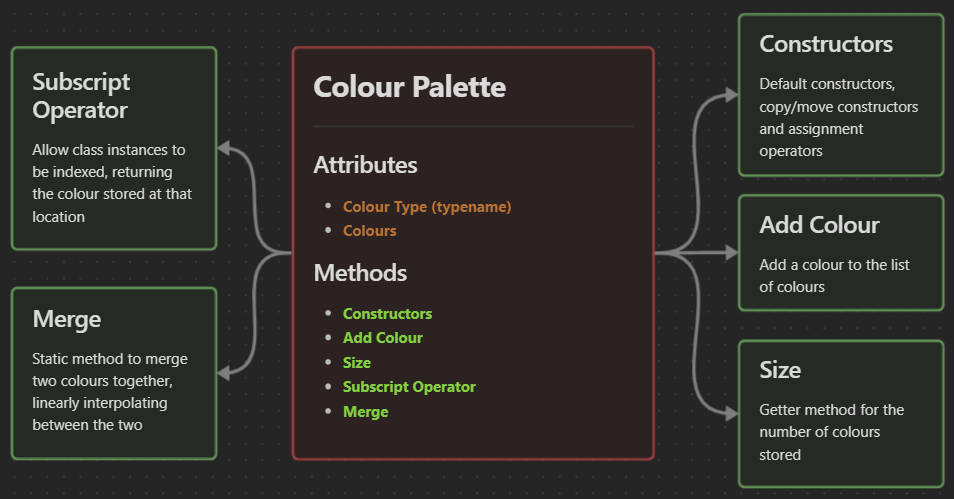
\includegraphics[width=\textwidth]{ClassColourPalette.png}
\end{figure*}
\FloatBarrier

The colour merging function is a very simple static method of the class, which linearly interpolates between the colour's red, green and blue components.

\begin{equation}
	\left\{ \phantom{\frac{a}{b}} t \times (R-r) + r, \quad t \times (G-g) + g, \quad t \times (B-b) + b \phantom{\frac{a}{b}} \right\}
\end{equation}

Where $t$ is the interpolation factor and $0 \le t \le 1$.

\subsection{The Fractal Class}

To support multiple fractal equations at runtime, each fractal will be implemented as a class inheriting from a main parent type. This is the fractal data type. It defines the functions required to iterate the fractal's equation from a given starting value, the logic to generate a colour from a starting point, an endpoint, and the number of iterations required to get there.

\FloatBarrier
\begin{figure*}[htp]
	\centering
	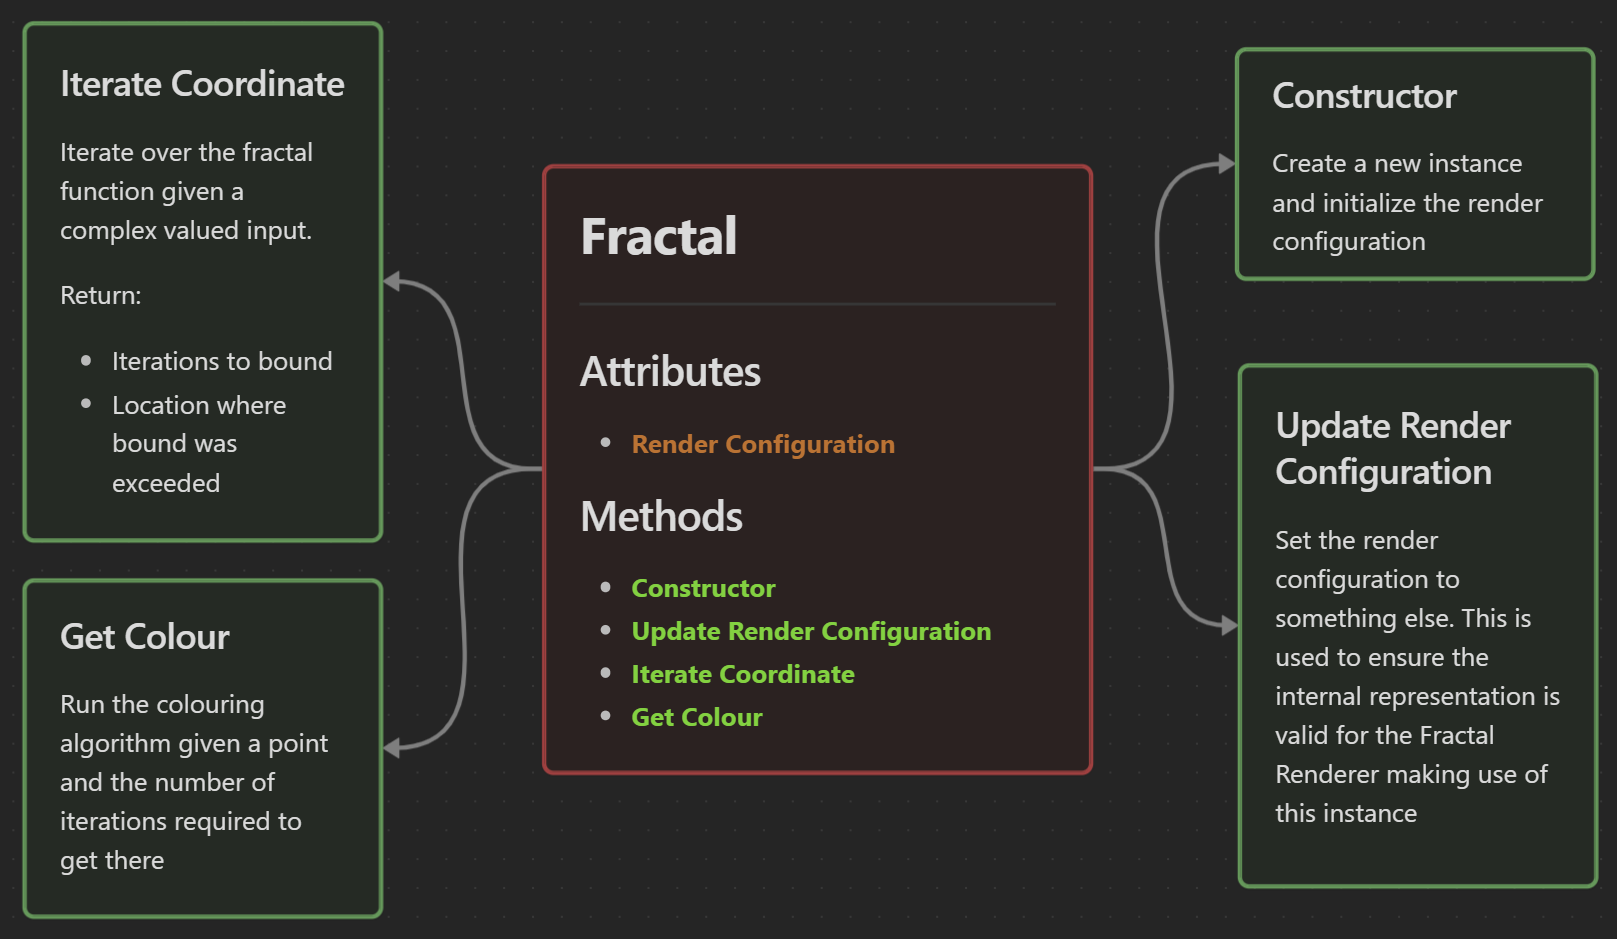
\includegraphics[width=\textwidth]{ClassFractal.png}
\end{figure*}
\FloatBarrier

\vspace{0.5cm}
\noindent
For example, the code below shows the definition of the Mandelbrot fractal class.

\begin{lstlisting}[language=c++]
	#pragma once
	
	#include <fractal/genericFractal.hpp>
	
	namespace frac {
		class Mandelbrot : public Fractal {
			public:
			/// Constructor taking a RenderConfig object
			/// \param config RenderConfig object
			explicit Mandelbrot(const RenderConfig &config);
			Mandelbrot(const Mandelbrot &)			  = delete;
			Mandelbrot(Mandelbrot &&)				  = delete;
			Mandelbrot &operator=(const Mandelbrot &) = delete;
			Mandelbrot &operator=(Mandelbrot &&)	  = delete;
			
			~Mandelbrot() override = default;
			
			LIBRAPID_NODISCARD std::pair<int64_t, lrc::Complex<LowPrecision>>
			iterCoordLow(const lrc::Complex<LowPrecision> &coord) const override;
			
			LIBRAPID_NODISCARD std::pair<int64_t, lrc::Complex<HighPrecision>>
			iterCoordHigh(const lrc::Complex<HighPrecision> &coord) const override;
		};
	} // namespace frac
\end{lstlisting}

\subsubsection{Render Box States}

An enum of valid states is required to keep track of each render box's current state. This is drawn to the main window on top of the fractal as it renders, providing the user with information about which areas are rendered, which are actively rendering and which areas are yet to be processed.

\begin{lstlisting}[language=c++]
	/// Represents the state of a render box
	enum class RenderBoxState {
		None,	   // Not yet assigned a state
		Queued,	   // Queued to be rendered
		Rendering, // Currently being rendered
		Rendered   // Rendered and ready to be written to the image
	};
\end{lstlisting}

\subsubsection{Render Boxes}

The position information required to render a small area of the main fractal is contained within a \codeword{RenderBox} struct. These can be passed to a function inside the \codeword{FractalRenderer} class to be processed. 

\begin{lstlisting}[language=c++]
	/// Stores the pixel-space coordinates of a region to render
	struct RenderBox {
		lrc::Vec2i topLeft;
		lrc::Vec2i dimensions;
		RenderBoxState state = RenderBoxState::None;
		double renderTime	 = 0;
	};
\end{lstlisting}

\subsubsection{Render Box Statistics}

To calculate the remaining time of the render and the fastest and slowest render box times, the program needs to know precisely how long each box took to render. To improve efficiency, a separate struct is created to store this data.

\begin{lstlisting}[language=c++]
	struct RenderBoxTimeStats {
		double min	  = 0;
		double max	  = 0;
		double average = 0;
		double remainingTime = 0;
	};
\end{lstlisting}

\subsubsection{Render Configurations}

Arguably the most important helper class, the \codeword{RenderConfig} struct, contains all the information required for a \codeword{FractalRenderer} instance to render an image. The information in this struct can also be saved to a JSON file and shared, allowing people to send specific configurations between users easily.

\begin{lstlisting}[language=c++]
	struct RenderConfig {
		int64_t numThreads; // Number of threads to render on (max)
		int64_t maxIters;	// Largest number of iterations to allow
		int64_t precision;	// Precision (in bits) of floating point types used for arithmetic
		LowPrecision bail;	// Bailout value
		int64_t antiAlias;	// Anti-aliasing factor -- 1 = no anti-aliasing
		lrc::Vec2i imageSize; // Size of the image to render
		lrc::Vec2i boxSize;	  // Size of sub-regions to render (see RenderBox)
		lrc::Vec<HighPrecision, 2> fracTopLeft;		 // The fractal-space center of the image
		lrc::Vec<HighPrecision, 2> fracSize;		 // The width and height of the fractal space
		lrc::Vec<HighPrecision, 2> originalFracSize; // Original size for zoom factor calculation
		ColorPalette palette; // The palette to use for rendering the fractal
	};
\end{lstlisting}

\subsection{The Fractal Renderer Class}

While it is essential to have a method of calculating the colour of a given point on the fractal (from the fractal class), it doesn't support rendering an entire image. This is the role of the fractal renderer class.

\FloatBarrier
\begin{figure*}[htp]
	\centering
	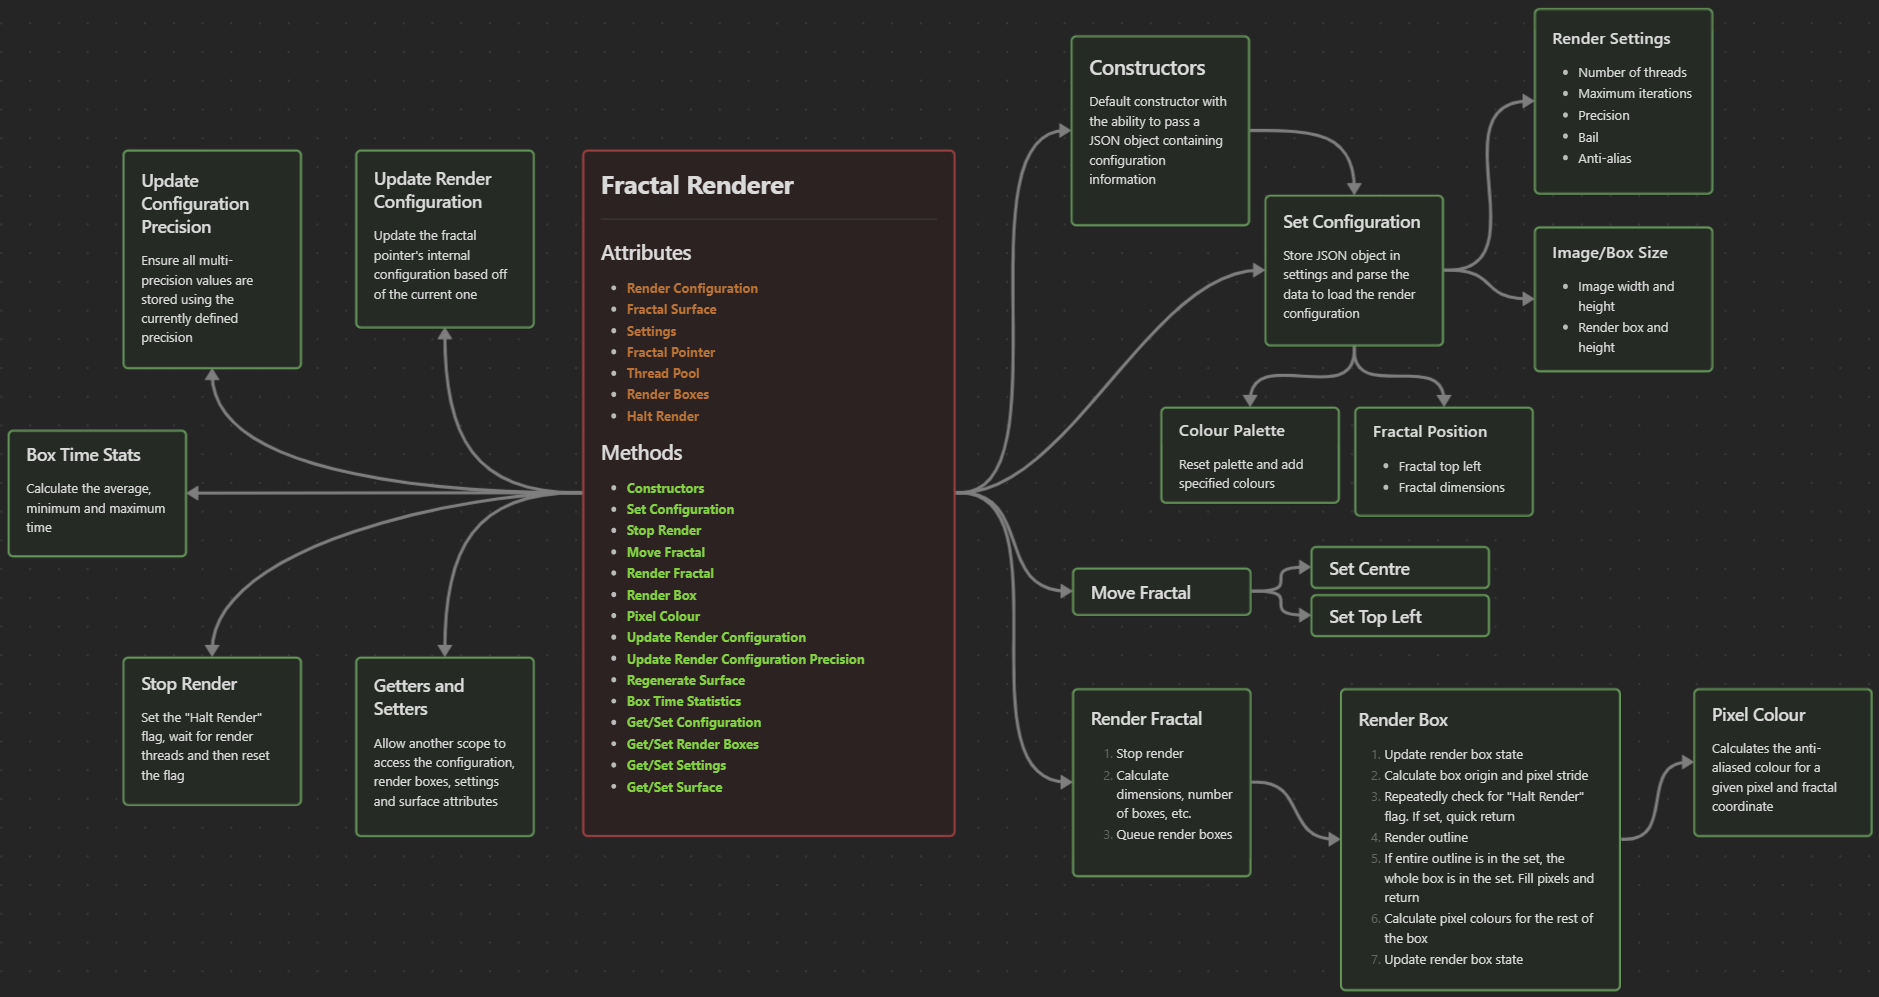
\includegraphics[width=\textwidth]{ClassFractalRenderer.png}
\end{figure*}
\FloatBarrier

This class implements many functions at various levels of abstraction, allowing performance-critical sections of the code to be run with efficient, parallelised algorithms. At the same time, the high-level interfaces are easy to interact with and use.

% Padding
\pagebreak

\subsubsection{Configuration, Getters, Setters and Statistics}

\FloatBarrier
\begin{figure*}[htp]
	\centering
	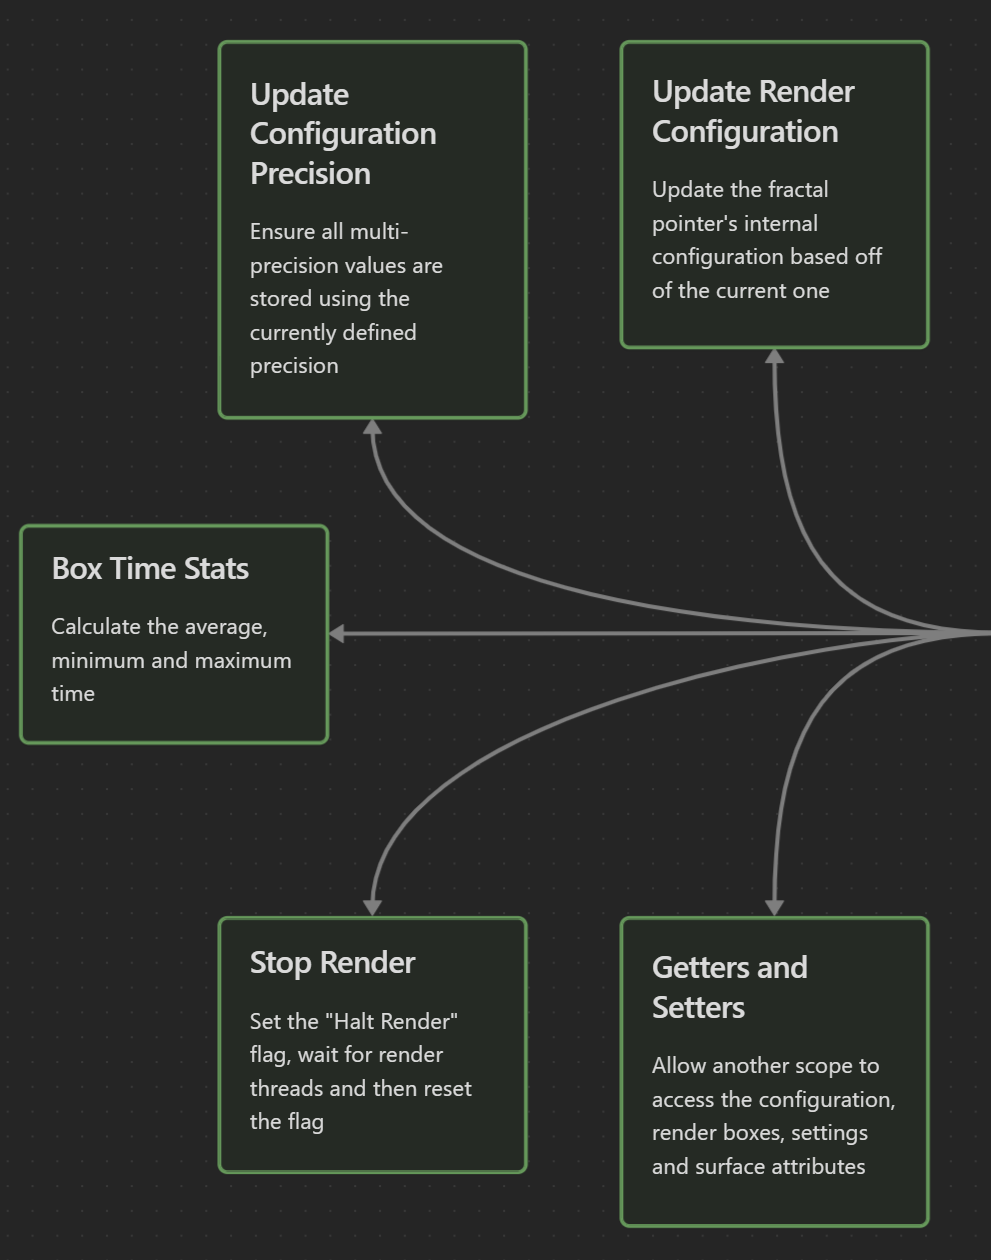
\includegraphics[width=.5\textwidth]{ClassFractalRendererLeftSide.png}
\end{figure*}
\FloatBarrier

These functions operate at a high level, allowing basic access to the information stored by the class. While simple, they are essential for the main program to function correctly, as there would be no way of accessing the rendered image, for example.

% Padding
\pagebreak

\subsubsection{Constructors and Configurations}

\FloatBarrier
\begin{figure*}[htp]
	\centering
	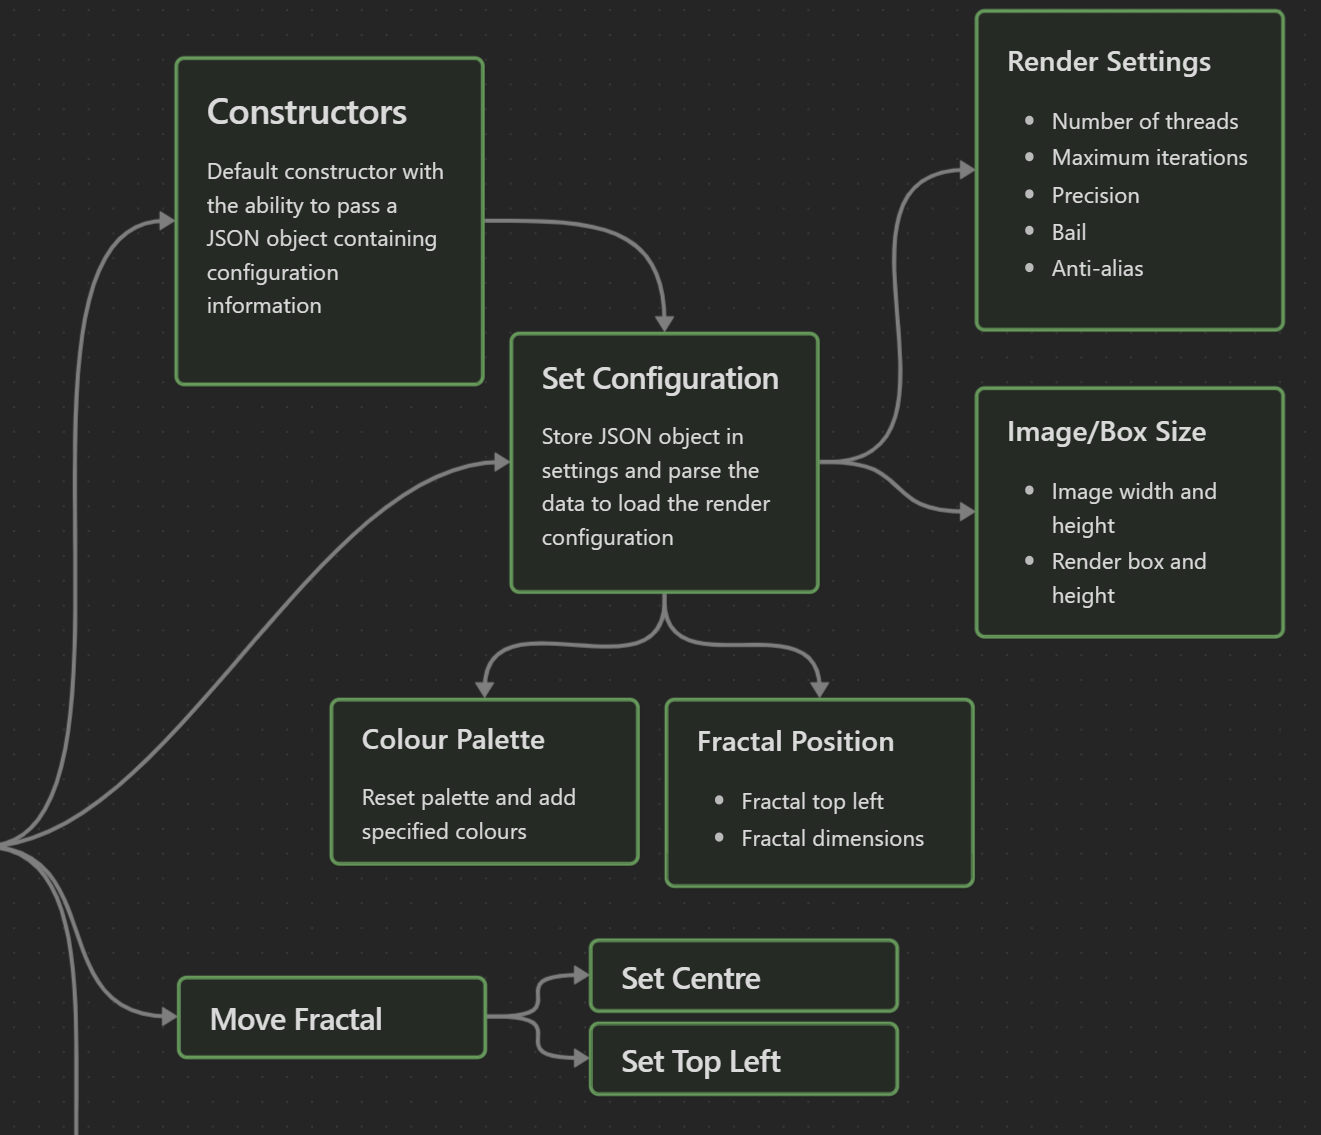
\includegraphics[width=\textwidth]{ClassFractalRendererTopRightSide.png}
\end{figure*}
\FloatBarrier

To render a fractal, much information is required about the dimensions of the image, the dimensions of the fractal, the origin in the complex plane, and more.

The fractal renderer class can parse a JSON object and load its configuration. By storing some data as a string instead of a number, it is possible to save and load high-precision numbers as well -- this could be used to enable fractal locations with extremely high zoom factors to be saved and shared easily.

\vspace{0.5cm}
\noindent
The JSON snippet below shows a highly simplified version of the default configuration used within the software (for a full version, see the code listing at the end of the document).

% Using language=python to change syntax highlighting
\begin{lstlisting}[language=python]
	{
		"renderConfig": {
			"numThreads": 8,
			"maxIters": 500,
			"precision": 64,
			"bail": 65536,
			"antiAlias": 2,
			"imageSize": {
				"width": 800,
				"height": 700
			},
			"colorPalette": [
			{
				"red": 0.5568628,
				"green": 0.23137255,
				"blue": 0.27450982,
				"alpha": 1.0
			},
			{
				"red": 0.88235295,
				"green": 0.8666667,
				"blue": 0.56078434,
				"alpha": 1.0
			}
			]
		}
	}
\end{lstlisting}

A vast number of configuration options can be configured in the file, including the threading options, render quality settings and even the size of the boxes to render in parallel.

The \codeword{loadConfiguration} method also enables the configuration to be changed or re-parsed at runtime, allowing quick and easy updates to the fractal settings.

\subsubsection{Rendering Algorithms}

\FloatBarrier
\begin{figure*}[htp]
	\centering
	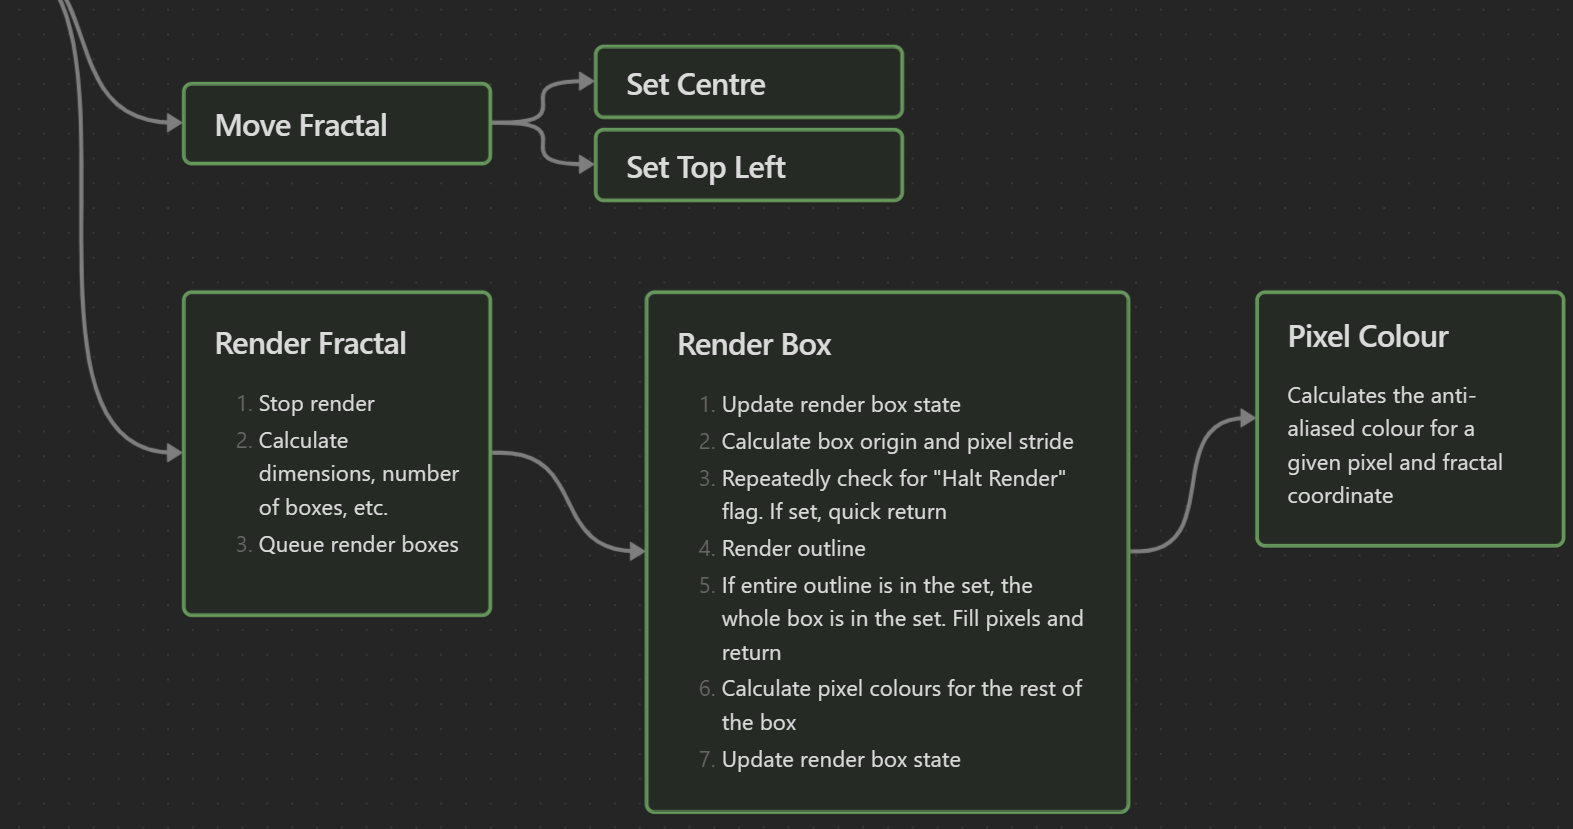
\includegraphics[width=\textwidth]{ClassFractalRendererBottomRightSide.png}
\end{figure*}
\FloatBarrier

The fractal renderer is responsible for creating an image buffer and setting the colour of each pixel in that image to represent the fractal at that location. Doing this efficiently is difficult, so the process is split into many small functions, providing fine-grained control over the algorithm.

\vspace{0.5cm}
\noindent
The following flowchart outlines the \codeword{renderFractal} method, which is explained in more detail below.
\vspace{0.5cm}

\begin{center}
	\begin{tikzpicture}[
		block/.style={rectangle, draw, text width=3.5cm, align=center, rounded corners},
		arrow/.style={->, >=stealth},
		node distance=0.75cm and 1cm
		]
		
		\node[block] (check) {Check if render already in progress};
		\node[block, below=of check] (halt) {Halt and wait for tasks to finish};
		\node[block, below=of halt] (log) {Write information to Log file};
		\node[block, below=of log] (reset) {Reset thread pool and clear render boxes};
		\node[block, below=of reset] (config) {Configure render parameters};
		\node[block, below=of config] (iterate) {Iterate over all boxes};
		\node[block, right=1cm of iterate] (createBox) {Create RenderBox};
		\node[block, right=1cm of createBox] (pushTask) {Push task to thread pool};
		\node[block, below=of iterate] (complete) {Render successfully started};
		
		\draw[arrow] (check) -- (halt);
		\draw[arrow] (halt) -- (log);
		\draw[arrow] (log) -- (reset);
		\draw[arrow] (reset) -- (config);
		\draw[arrow] (config) -- (iterate);
		\draw[arrow] (iterate) to [bend right] (createBox);
		\draw[arrow] (createBox) to [bend right] (pushTask);
		\draw[arrow] (pushTask) to [bend right] (iterate);
		\draw[arrow] (iterate) -- (complete);
	\end{tikzpicture}
\end{center}

Upon requesting the renderer to re-render the image, any existing render threads are halted, dependent image settings are recalculated, and the render-box queue is cleared.

Next, the render boxes are recalculated and pushed back to the render queue. Each box is dequeued by a thread in a thread pool and runs in parallel.

To optimise the rendering of each box, we can use the fact that if an outline can be drawn where every point is in the set, every point contained within that outline must also be within the set. Outlining each box before calculating the inner area makes it possible to check whether all points were in the set. If they were, we can quickly fill the rest of the box without calculating the colour of each pixel.

\begin{center}
	\begin{tikzpicture}[
		block/.style={rectangle, draw, text width=4.0cm, align=center, rounded corners},
		arrow/.style={->, >=stealth},
		node distance=1.5cm and 1.5cm
		]
		
		\node[block] (initVars) {Initialize variables};
		\node[block, below=of initVars] (checkOptimisation) {Does this fractal support optimisations?};
		\node[block, right=of checkOptimisation] (renderEdges) {Render the edges of the box};
		\node[block, below=of renderEdges] (checkEdges) {Were all edges in the set?};
		\node[block, below=of checkEdges] (blackBox) {Fill the whole box black};
		\node[block, left=of checkEdges] (renderBox) {For each pixel, find its color};
		\node[block, left=of blackBox] (update) {Update the \codeword{RenderBox} information};
		
		\draw[arrow] (initVars) -- (checkOptimisation);
		\draw[arrow] (checkOptimisation) -- node[anchor=south]{Yes} (renderEdges);
		\draw[arrow] (checkOptimisation) -- node[anchor=west]{No} (renderBox);
		\draw[arrow] (renderEdges) -- (checkEdges);
		\draw[arrow] (checkEdges) -- node[anchor=south]{No}(renderBox);
		\draw[arrow] (checkEdges) -- node[anchor=east]{Yes}(blackBox);
		\draw[arrow] (renderBox) -- (update);
		\draw[arrow] (blackBox) -- (update);
	\end{tikzpicture}
\end{center}

To calculate the colour of each pixel, we first call the \codeword{iterCoord} method of the fractal pointer stored to get the number of iterations required to exceed the bailout value (if it is exceeded at all), as well as the first point at which this occurs. This information is then passed to the fractal's colouring algorithm to generate a colour for the pixel. If anti-aliasing is enabled, this process is repeated for multiple points within the pixel, and the resulting colours are averaged. Anti-aliasing produces smoother images that appear to be higher resolution, allowing for faster render times with high-quality results.

\vspace{0.5cm}

The fractal renderer class also implements routines to change the fractal-space coordinates to render. This is used to move the fractal when zooming in or out. For different use cases, there are methods to set the top left coordinate or the image's centre.

% Padding
\pagebreak

\subsection{The Main Window}

\FloatBarrier
\begin{figure*}[htp]
	\centering
	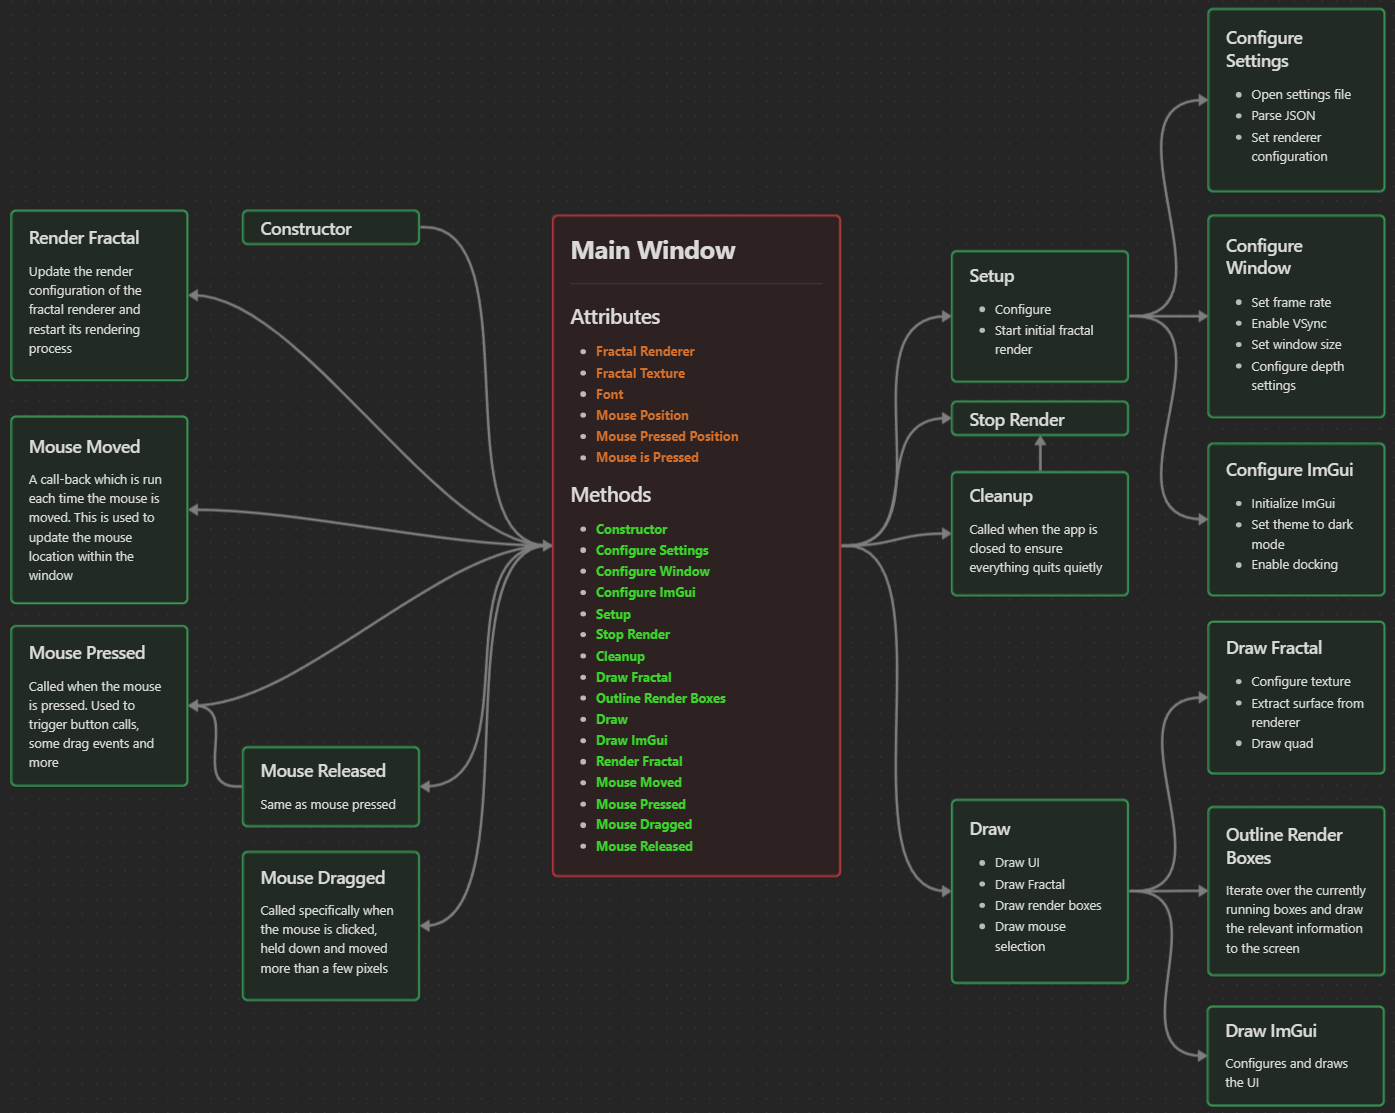
\includegraphics[width=\textwidth]{ClassMainWindow.png}
\end{figure*}
\FloatBarrier

This class is responsible for creating, managing and drawing information to the window and controlling all the other classes mentioned previously.

\vspace{0.5cm}
\noindent
When the window is created by \textit{Cinder}, the \codeword{setup} routine is called, initializing the window's attributes. First, the settings JSON file is loaded, parsed and passed to the fractal renderer member. Next, the window itself is constructed and configured, including the framerate, enabling or disabling vertical syncing (V-Sync), the window size and OpenGL depth buffer settings. Finally, \textit{ImGui} is configured.

The \codeword{MainWindow} class is also responsible for drawing to the window. After setting the background colour, the \textit{ImGui} windows are created and drawn. This produces most of the UI, but some extra parts must be drawn in later. Next, the fractal itself is drawn to the screen. An image texture is created and assigned the fractal image buffer, and a rectangle is drawn with the aforementioned texture. The rest of the UI is now drawn, including the render-box status indicators and the mouse selection.

When the application is requested to close, the \codeword{cleanup} routine is called. This signals any existing render threads to halt, ensures all members are correctly destructed and then destroys the window.

The window also has a variety of callback functions which are called when specific triggers occur. For example, functions are called every time the mouse is moved, dragged or pressed.

\subsection{Supporting Multiple Fractals and Colouring Algorithms}

Adding support for more fractal types and colouring algorithms is complicated and requires a significant rewrite of the current program. The reasons for this are non-trivial, but, in essence, it's mainly due to the iterative equations and colouring algorithms required for each fractal type. For example, the Mandelbrot set can be optimised in ways that Newton's fractal cannot and is generally coloured with completely different methods.

\subsubsection{Altering the Main Rendering Loop}

While many optimisations are possible when rendering fractals, the simplest and most effective one (for the fractals that apply) relies on the fact that if a complete outline can be drawn where every point is known to be contained within the set, every point within that border must also be within the set. This applies to the Mandelbrot set and many variations of it but not, for example, Newton's fractal.

Each fractal type must provide a method of defining what optimisations are available for it so the rendering algorithm can produce a precise, artefact-free image. Although the software will only implement a single optimisation method, support for up to 64 will be implemented. This future-proofs the application and simplifies the addition of more optimal algorithms in the future. The code below shows some snippets from the source code that enable this.

\begin{lstlisting}[language=c++]
	namespace optimisations {
		constexpr size_t OUTLINE_OPTIMISATION = 0x0001;
	}
	
	// ------------------------------------------------
	
	virtual size_t supportedOptimisations() const;
	
	// ------------------------------------------------
	
	const size_t supportedOptimisations = m_fractal->supportedOptimisations();
	const bool supportsOutlining =
	supportedOptimisations & optimisations::OUTLINE_OPTIMISATION;
\end{lstlisting}

\subsubsection{Implementing More Colouring Algorithms}

Using the previous example of Newton's fractal and the Mandelbrot set, it is clear that the algorithms used to colour them are very different. Unfortunately, this means that the class structure outlined previously will not work. Instead of the \codeword{Fractal} class implementing colouring algorithms, they will instead implement a method which returns a dictionary of valid algorithms for each fractal. The key will be the algorithm's name, and the value will be a function pointer or lambda. This way, creating an ImGui window to change the algorithm at runtime is significantly easier.

A drop-down menu is created to select the colouring algorithm, showing the keys in the colour mapping dictionary. When the user selects one of the items in the list, the colouring algorithm is updated to the function specified by that key and the fractal is re-rendered.

\subsubsection{Supporting Multiple Colour Schemes}

Adding support for colour schemes and palettes involves a process similar to adding more colouring algorithms. The valid colour palettes are loaded from the JSON configuration file and shown in a dropdown list, where the user can then select the desired palette. The palette is loaded into the program, and the fractal is re-rendered to show the changes.

\vspace{0.25cm}
\noindent
The colour palettes are defined in the JSON file with the following structure.
\begin{lstlisting}[language=python]
	{
		...
		"colorPalettes": [
		{
			"name": "My Palette",
			"colors": [
			{
				"red": 0.5,
				"green": 0.5,
				"blue": 0.5,
				"alpha": 1
			}
			]
		},
		...
		]
		...
	}
\end{lstlisting}

\subsubsection{Adding More Fractals}

Creating a new fractal type is very simple and can be achieved by writing a new class which inherits from the generic \codeword{Fractal} base class. The class must then be inserted into the software.

A window with a dropdown menu allows the user to change the currently rendered fractal. The flowchart shown below outlines the logic for the selection process. The fractal must also be added to the \codeword{settings.json} file, which contains the default configuration for that particular fractal.

\begin{center}
	\begin{tikzpicture}[node distance=2cm, align=center]
		\node (start) [boxNode] {Start};
		\node (in1) [boxNode, below of=start, node distance=2cm] {Input: name};
		\node (dec1) [boxNode, below of=in1, minimum width=4cm, minimum height=1.8cm, node distance=3cm] {name is \\ ``Mandelbrot"};
		\node (proc1) [boxNode, right of=dec1, node distance=6cm, minimum width=6cm] {newFracPtr = Mandelbrot};
		\node (dec2) [boxNode, below of=dec1, node distance=3cm, boxNode, below of=in1, minimum width=4cm, minimum height=1.8cm] {name is \\ ``Julia Set"};
		\node (proc2) [boxNode, right of=dec2, node distance=6cm, minimum width=6cm] {newFracPtr = JuliaSet};
		\node (dec3) [boxNode, below of=dec2, node distance=3cm, boxNode, minimum width=4cm, minimum height=1.8cm] {name is \\ ``Newton's Fractal"};
		\node (proc3) [boxNode, right of=dec3, node distance=6cm, minimum width=6cm] {newFracPtr = NewtonFractal};
		\node (proc4) [boxNode, below of=dec3, yshift=-0.5cm] {Clear history};
		\node (proc5) [boxNode, below of=proc4] {Update Fractal\\Pointer Type};
		\node (stop) [boxNode, below of=proc5] {End};
		
		\draw [arrow] (start) -- (in1);
		\draw [arrow] (in1) -- (dec1);
		\draw [arrow] (dec1) -- node[anchor=south] {yes} (proc1);
		\draw [arrow] (dec1) -- node[anchor=east] {no} (dec2);
		\draw [arrow] (proc1) -| ([xshift=1cm]proc1.east) |- (proc4);
		\draw [arrow] (dec2) -- node[anchor=south] {yes} (proc2);
		\draw [arrow] (dec2) -- node[anchor=east] {no} (dec3);
		\draw [arrow] (proc2) -| ([xshift=1cm]proc2.east) |- (proc4);
		\draw [arrow] (dec3) -- node[anchor=south] {yes} (proc3);
		\draw [arrow] (dec3) -- node[anchor=east] {no} (proc4);
		\draw [arrow] (proc3) -| ([xshift=1cm]proc3.east) |- (proc4);
		\draw [arrow] (proc4) -- (proc5);
		\draw [arrow] (proc5) -- (stop);
	\end{tikzpicture}
\end{center}



\subsection{Additional Features}

The features outlined previously comprise the vast majority of the program, but some additional features must also be designed and implemented. These are often the less critical features, though they still impact the user's interaction with the program.  

\subsubsection{Movement History}

While we often take the ``undo'' and ``redo'' buttons for granted, they give us a powerful means of reverting unwanted changes. Furthermore, they allow the user to see what adjustments have been made to the fractal between movements, supporting verbal descriptions of how to arrive at fascinating points within the fractal.

Using a linked list, where each node stores a \codeword{RenderConfig} object and a \codeword{Surface}, it is possible to implement a history into the program. Whenever the user requests to change a setting or move the origin of the fractal, the current surface and render configuration are appended to the history before the changes are applied. The algorithm to append to the linked list can be seen below.

\begin{center}
	\begin{tikzpicture}
		\node (classDef) [boxNode] {
			$
			\begin{aligned}
				&\textbf{HistoryNode} \\ \\
				&\codeword{HistoryNode *m_next} \\
				&\codeword{HistoryNode *m_prev} \\
			\end{aligned}
			$
		};
		\node (appendFn) [boxNode, below of = classDef, node distance = 100pt] {
			$
			\begin{gathered}
				\codeword{append(HistoryNode *node)}
			\end{gathered}
			$
		};
		\node (ifStatement) [conditionNode, below of = appendFn, node distance = 100pt] {
			$
			\begin{gathered}
				\codeword{m_next} \text{ is } \codeword{NULL}?
			\end{gathered}
			$
		};
		
		\node (ifPoint) [square, right of = ifStatement, node distance = 180pt] {no};
		
		\node (recurse) [boxNode, right of = appendFn, node distance = 180 pt] {
			$
			\begin{gathered}
				\text{Call } \codeword{append} \text{ on } \codeword{m_next}
			\end{gathered}
			$
		};
		
		\node (assignStatement) [boxNode, below of = ifStatement, node distance = 100pt] {
			$
			\text{Assign } \codeword{node} \text{ to } \codeword{m_next}
			$
		};
		
		\node (assignStatement2) [boxNode, right of = assignStatement, node distance = 170pt] {
			$
			\text{Assign } \codeword{*this} \text{ to } \codeword{m_next->m_prev}
			$
		};
		
		\draw [arrow] (classDef) -- (appendFn);
		\draw [arrow] (appendFn) -- (ifStatement);
		\draw (ifStatement) -- (ifPoint);
		\draw [arrow] (ifPoint) -- (recurse);
		\draw [arrow] (recurse) -- (appendFn);
		\draw [arrow] (ifStatement) -- node[anchor = east]{yes} (assignStatement);
		\draw [arrow] (assignStatement) -- (assignStatement2);
	\end{tikzpicture}
\end{center}

\vspace{2cm}

The \codeword{MainWindow} class also stores a pointer to the current node in the history buffer. Using this, it is possible to detect whether there are changes before or after the current node by checking the validity of the \codeword{previous} and \codeword{next} pointers, respectively.

When the user makes a change, the current node is checked against the end of the history buffer. If there are no changes after the current state, the new state is appended directly to the end of the buffer. However, if changes exist, destroying the rest of the tree with the \codeword{killChildren} method is necessary before appending the new configuration. To undo moves, the current node is moved back down the list.

To make these commands as intuitive as possible, the undo and redo operations are triggered by pressing \codeword{ctrl+z} and \codeword{ctrl+shift+z}, respectively. These are very common commands and will be easy to remember.

To show the user the current history, a small tab is rendered on the right side of the window. Each item in the history buffer is shown by drawing the saved surface, with the current item outlined to make it more obvious where in the history tree you are.

Mouse events within this tab are also supported, such as scrolling and clicking on frames to select items in the history.

Scrolling is implemented with a single offset that increases or decreases as the mouse wheel moves. The rate at which the window scrolls is defined by the \codeword{settings[`menus'][`history'][`scrollSpeed']} value in the settings JSON file.

\subsubsection{Improved Selection Area}

To improve the user interface, the zoom selection box should not zoom in immediately after being drawn. Once the box is specified, it should be possible to drag it around to specify where the zoom will occur more precisely. Keyboard inputs (such as the arrow keys) should also move the selected region.

Adding the mouse position delta to the box's position keeps the box in the same place relative to the mouse, enabling it to be dragged by the user. The code below shows a simple implementation.

\begin{lstlisting}[language=c++]
	void MainWindow::mouseDrag(ci::app::MouseEvent event) {
		if (ImGui::GetIO().WantCaptureMouse) return;
		
		lrc::Vec2i delta = lrc::Vec2i(event.getPos()) - m_mousePos;
		m_mousePos		 = event.getPos();
		
		if (m_moveZoomBox) {
			m_zoomBoxStart += delta;
			m_zoomBoxEnd += delta;
		}
	}
\end{lstlisting}

Moving the zoom area with the arrow keys requires a switch-case block to check which key has been pressed.

\begin{lstlisting}[language=c++]
	switch (event.getCode()) {
		case ci::app::KeyEvent::KEY_RETURN: {
			zoomFractal(m_zoomBoxStart, m_zoomBoxEnd);
		}
		case ci::app::KeyEvent::KEY_ESCAPE: {
			m_showZoomBox = false;
			break;
		}
		case ci::app::KeyEvent::KEY_RIGHT: {
			m_zoomBoxStart.x(m_zoomBoxStart.x() + scrollSpeed);
			m_zoomBoxEnd.x(m_zoomBoxEnd.x() + scrollSpeed);
			break;
		}
		case ci::app::KeyEvent::KEY_LEFT: {
			m_zoomBoxStart.x(m_zoomBoxStart.x() - scrollSpeed);
			m_zoomBoxEnd.x(m_zoomBoxEnd.x() - scrollSpeed);
			break;
		}
		case ci::app::KeyEvent::KEY_UP: {
			m_zoomBoxStart.y(m_zoomBoxStart.y() - scrollSpeed);
			m_zoomBoxEnd.y(m_zoomBoxEnd.y() - scrollSpeed);
			break;
		}
		case ci::app::KeyEvent::KEY_DOWN: {
			m_zoomBoxStart.y(m_zoomBoxStart.y() + scrollSpeed);
			m_zoomBoxEnd.y(m_zoomBoxEnd.y() + scrollSpeed);
			break;
		}
	}
\end{lstlisting}

\subsubsection{Enabling Window Resizing}

If the program is resized, the image should continue to be drawn at the largest size possible, and all existing operations should remain fully functional. The main consequence is the requirement to map various coordinates from screen space to image space and vice-versa. For example, the zoom box must be scaled so that when the pixels in the image do not align perfectly with the pixels on the screen, the correct area is still zoomed into. This is achieved by multiplying the coordinate/vector by a scaling factor.

\begin{equation*}  \label{screenToImageSpace}
	\begin{bmatrix} x' \\ y' \end{bmatrix} = \frac{\text{Image Height}}{\text{Window Height}} \begin{bmatrix} x \\ y \end{bmatrix}
\end{equation*}

Resizing the image leads to additional aliasing in the rendering process since the pixels of the image do not align perfectly with those of the screen. This can be fixed by allowing the user to resize the image to the current window size.

\begin{lstlisting}[language=c++]
	ImGui::SameLine();
	if (ImGui::Button("Reset Image Size")) {
		stopRender();
		config.imageSize = imageToScreenSpace(config.imageSize);
		m_renderer.regenerateSurface();
		renderFractal();
	}
\end{lstlisting}

Note that, in the above code snippet, the \codeword{imageToScreenSpace} function performs the inverse of the \codeword{screenToImageSpace} function described earlier (\ref{screenToImageSpace}).

\begin{equation*}
	\begin{bmatrix} x \\ y \end{bmatrix} = \frac{\text{Window Height}}{\text{Image Height}} \begin{bmatrix} x' \\ y' \end{bmatrix}
\end{equation*}

\subsection{Importing and Exporting Configurations}

Arguably the most crucial feature of this program is the ability to import and export detailed fractal configuration information. This enables users to share reproducible fractal locations, colouring algorithms and palettes.

To export the settings, the current render configuration must be written back to the JSON object that was initially loaded. The JSON object can be dumped into a file when this is complete.

Importing the settings JSON file is very easy, given the renderer already provides a method to open a JSON file, parse the input and initialize the renderer.

Additionally, a GUI window is needed to allow the user to specify where to save the file. A text box is shown with a prompt for a file path, and the entered string is checked against a list of valid extensions. If the extension is valid, two buttons are shown -- one for exporting the configuration and one for importing it. If the file path was invalid or an error occurred at some point, the program will handle the error appropriately and log it using the \codeword{DebugLogger} class.

\subsection{Saving Rendered Images}

Saving the image is very simple since it is stored in the \codeword{FractalRenderer} instance of the \codeword{MainWindow}, and Cinder provides methods to save surfaces as image files.

As with the configuration import and export, the input box checks for valid image extensions and only shows the export button if a valid path is entered. Similarly, the information is written to the log file if an error occurs, and the program will continue running.
